\documentclass[12pt]{exam}
\usepackage[phy]{template-for-exam}
\usepackage{pgfplots}
\pgfplotsset{
  compat=1.18,
  width=6cm,
  posgraph/.append style={
    axis y line = left,
    axis x line = center,
    axis line style = ultra thick,
    xlabel={\bf time},
    ylabel={\bf displacement},
    ymin=0,
    ymax=9,
    xmin=0,
    xmax=3,
    xtick=\empty,
    ytick=\empty,
  },
  velgraph/.append style={
    xlabel={\bf time},
    ylabel={\bf velocity},
    ymin=-5,
    ymax=5,
    xmin=0,
    xmax=4,
    ytick=\empty,
    xtick=\empty,
    axis y line = left,
    axis x line = center,
    axis line style = ultra thick,
  },
  numberedplots/.append style={
    xlabel={\bf time (s)},
    width=7cm,
    ytick={-15,...,15},
    xtick={0,...,5},
    axis y line = left,
    axis x line = center,
    grid=major,
    axis line style = ultra thick,
  },
}
\usepackage{multicol}
\usepackage{graphicx}


\newcommand{\graphquestions}{
  \begin{subparts}
    \subpart
      The object is moving

      \begin{oneparcheckboxes}
        \choice forward
        \choice backward
      \end{oneparcheckboxes}

    \subpart
      The object is

      \begin{oneparcheckboxes}
        \choice speeding up
        \choice slowing down
        \choice moving at a constant speed
      \end{oneparcheckboxes}

    \subpart
      Calculate the velocity (if possible).
      \vspace{.75cm}

    \subpart
      Calculate the acceleration.
      \vspace{.75cm}


  \end{subparts}
}

\newcommand{\blankgraphs}{
  \begin{multicols}{2}

    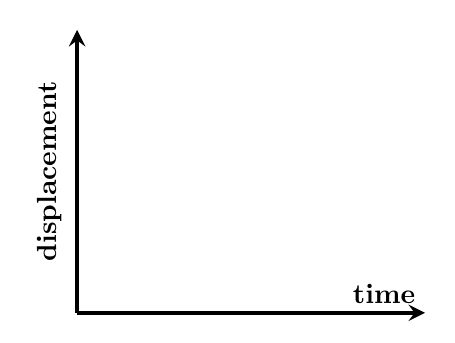
\begin{tikzpicture}
      \begin{axis}[posgraph]
      \end{axis}
    \end{tikzpicture}

    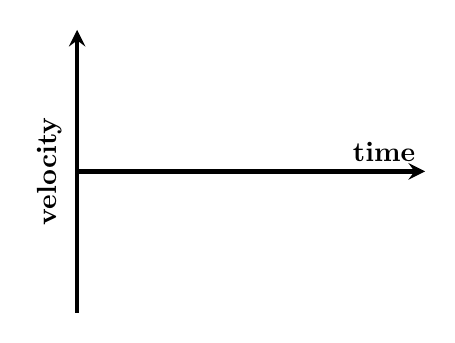
\begin{tikzpicture}
      \begin{axis}[velgraph]
      \end{axis}
    \end{tikzpicture}
    
  \end{multicols}
}


\title{Motion \#5}
\author{Rohrbach}


\begin{document}
\maketitle

\begin{questions}

\question
  For each of the following graphs, answer the 
  accompanying questions.

  \begin{parts}
    \part
    Consider this graph and answer the questions

      \begin{multicols}{2}

        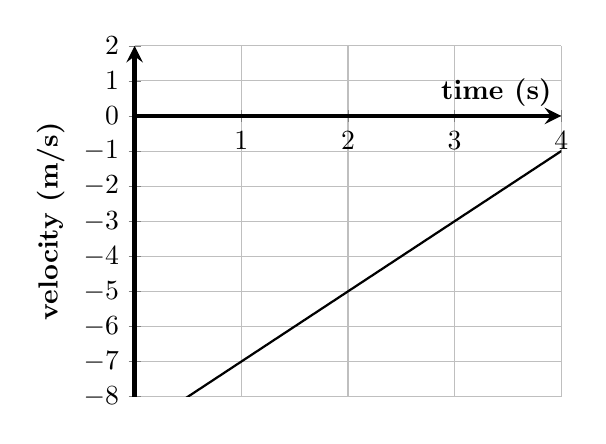
\begin{tikzpicture}
          \begin{axis}[
            numberedplots,
            ylabel={\bf velocity (m/s)},
            width=7cm,
            ymin=-8,
            ymax=2,
            xmin=0,
            xmax=4,
          ]
          \addplot[smooth,thick]{2*x-9};
         \end{axis}
       \end{tikzpicture}

       \graphquestions
       
      \end{multicols}




    \part
    Consider this graph and answer the questions

      \begin{multicols}{2}

        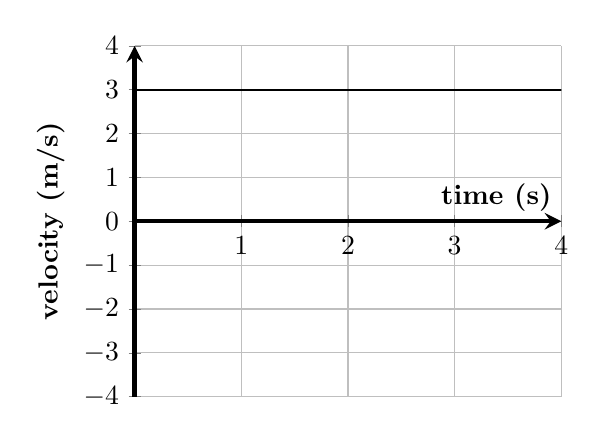
\begin{tikzpicture}
          \begin{axis}[
            numberedplots,
            ylabel={\bf velocity (m/s)},
            ymin=-4,
            ymax=4,
            xmin=0,
            xmax=4,
          ]
          \addplot[smooth,thick]{3};
          \end{axis}
        \end{tikzpicture}

        \graphquestions
        
      \end{multicols}

    \part
      {\bf Be careful!  This is a \emph{displacement} graph.}
    
      \begin{multicols}{2}

        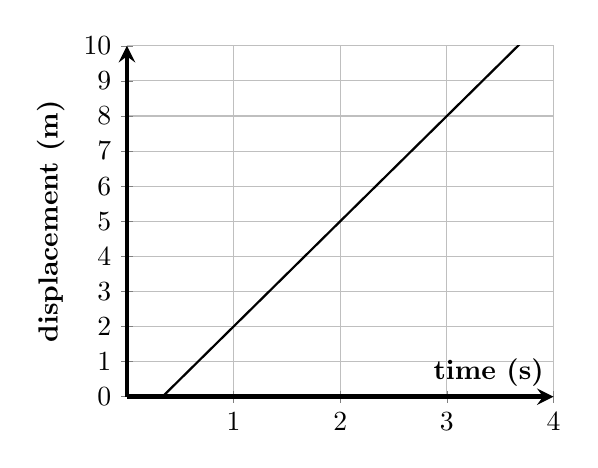
\begin{tikzpicture}
          \begin{axis}[
            numberedplots,
            ylabel={\bf displacement (m)},
            ymin=0,
            ymax=10,
            xmin=0,
            xmax=4,
          ]
          \addplot[smooth,thick]{3*x-1};
          \end{axis}
        \end{tikzpicture}

        \graphquestions
        
      \end{multicols}
  \end{parts}

\pagebreak

\question
  What is the difference between the motion of these 
  two objects?

  \begin{multicols}{2}

    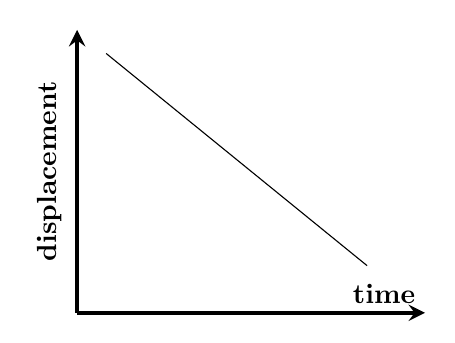
\begin{tikzpicture}
      \begin{axis}[posgraph]
      \addplot[smooth,domain=0.25:2.5]{-3*x+9};
      \end{axis}
    \end{tikzpicture}

    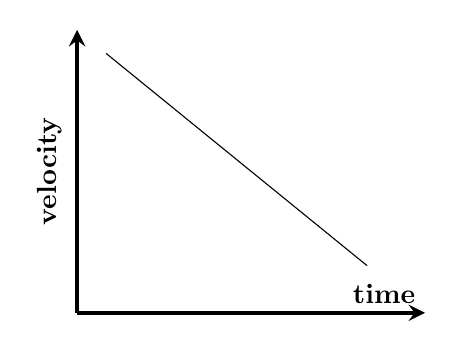
\begin{tikzpicture}
      \begin{axis}[
        posgraph,
        ylabel={\bf velocity}
      ]
      \addplot[smooth,domain=0.25:2.5]{-3*x+9};
      \end{axis}
    \end{tikzpicture}
    
  \end{multicols}

\question
  Draw the position and velocity graphs for each of 
  the following situations

  \begin{parts}
    
    \part
      Going backward at a constant speed.
      \blankgraphs

    \part
      Going forward and speeding up.
      \blankgraphs

    \part
      Going backward and speeding up.
      \blankgraphs


  \end{parts}

\end{questions}
\end{document}
